\documentclass[12pt,twoside]{article}
\usepackage{../jmlda}
\usepackage{mathtools}
\usepackage{lineno}
\usepackage{setspace}
\usepackage{graphicx}
\linenumbers
\doublespacing
%\NOREVIEWERNOTES
\title
    [Прогнозирование намерений]
    {Прогнозирование намерений. Исследование свойств локальных моделей при пространственном декодировании сигналов головного мозга.}
\author
    {Болоболова~Н.\,А., Мокропуло~Ю.\,И., Самохина~А.\,М., Шиянов~В.\,А.,}
\thanks
    {Работа выполнена при финансовой поддержке РФФИ, проект \No\,00-00-00000.
    Научный руководитель:  Стрижов~В.\,В.
    Задачу поставил: Стрижов~В.\,В.
    Консультант: Исаченко~Р.\,О.}
%\organization
%    {$^1$Организация; $^2$Организация}
\abstract
    {В данной работе исследуются механизмы регуляции движения конечностей нейронами головного мозга. Проверяется гипотеза о влиянии перемещения зон активности нейронов на траекторию движения конечности. Высокая размерность признакового пространства сигналов приводит к неустойчивости модели машинного обучения. Сигнал высокой размерности предлагается аппроксимировать локальной моделью, что существенно уменьшает размерность пространства параметров. Пространство параметров локальной модели используется как признаковое пространство. Таким образом, результирующая модель становится проще и устойчивее. В задаче используются данные электрокортикограмм, собранные на основе исследований активности нейронов головного мозга обезьян.    	

\bigskip
\textbf{Ключевые слова}: \emph{Brain-Computer Interface (BCI), feature engineering}.}
\begin{document}
\maketitle
\bigskip
\bigskip
\bigskip
\bigskip
\bigskip
\maketitleSecondary

\section{Введение}
Нейрокомпьютерный интерфейс (Brain Computer Interface) \cite{Morishita2014} позволяет восстановить мобильность людей с нарушениями двигательных функций.  Алгоритм BCI транслирует сигналы нейронов головного мозга в команды для исполняющей системы \cite{Morishita2014}. Это дает возможность регулировать движение роботизированной конечности в соответствии с механизмами нервной регуляции. \cite{Donoghue2008}. \\
Активность нейронов представляет собой временные вспышки сигналов различной интенсивности, их суперпозицию и распространение. Каждый канал имеет доступ к сигналам некоторого количества нейронов, находящихся в небольшой области пространства. Каждый нейрон соединен с помощью множества отростков с приблизительно 20 тысячами других нейронов. Именно эти сигналы представляют собой активность мозга.\\
В последнее время большое количество работ посвящено методам считывания мозговой активности и декодирования информации \cite{Hu2018,Song2017,Loza2017,Eliseyev2016,Gaglianese2016,Bundy2016,Morishita2014}.
В этой работе используются данные сигналов, полученных инвазивным методом электрокортикографии (ECoG) \cite{Sirven2014}. Сложность задачи заключается в избыточной размерности сигнала. Модель прогнозирования намерений является неустойчивой. Для построения устойчивой модели необходимо построить удобное признаковое пространство.\\
Исследование состоит в восстановлении зависимостей между сигналами ECoG и движениями конечностей. Для точного предсказания траектории движения в трехмерном пространстве требуется снизить размерность признакового пространства.\\
Стандартные подходы состоят в извлечении информативных признаков из пространственных, частотных и временных характеристик сигнала\cite{Morishita2014,Alexander2013}. Большинство методов в смежных работах исследуют частотные характеристики\cite{Chin2007,Eliseyev2014,Loza2017}. В работах \cite{Eliseyev2016,Motrenko2018} рассматриваются все признаки вне зависимости от их природы. Наиболее распространёнными моделями являются алгоритмы PLS\cite{Rosipal2006,Eliseyev2016}, PCA\cite{Zhao2010,Song2017}. В работе \cite{Zhao2014} используются алгоритмы, построенные на скрытых марковских моделях. В  работах \cite{Loza2017,Song2017} авторы рассматривают различные участки сигнала в виде слов. В работе \cite{Motrenko2018} исследован метод отбора признаков с помощью квадратичного программирования (Quadratic Programming Feature Selection \cite{rodriguez2010quadratic}).\\
\begin{figure}
\begin{center}
	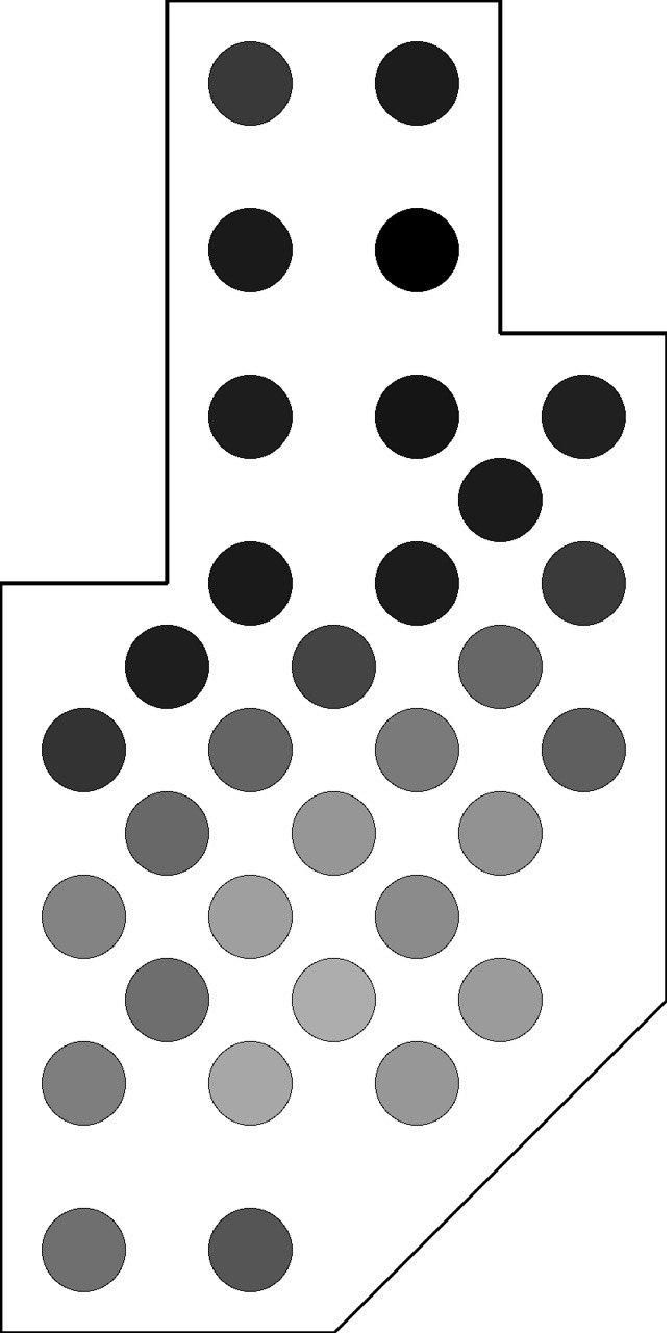
\includegraphics[width=100pt,height=\textheight,keepaspectratio]{wave0.pdf}
	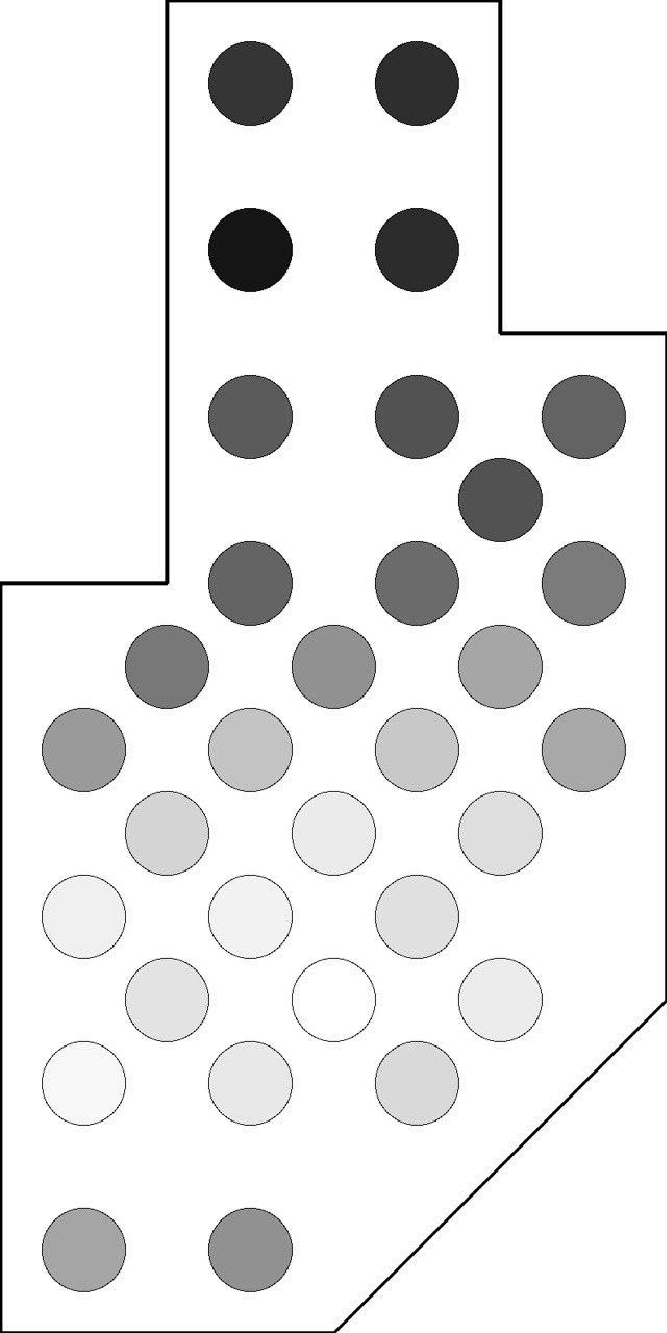
\includegraphics[width=100pt,height=\textheight,keepaspectratio]{wave1.pdf}
	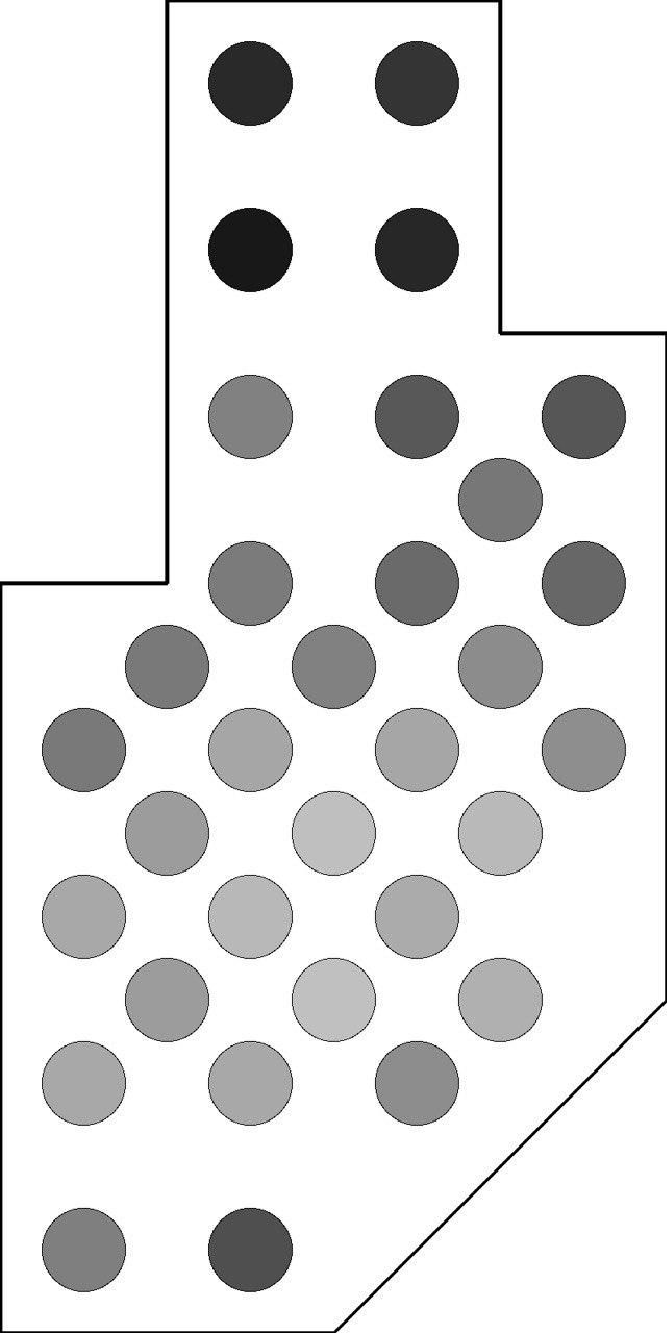
\includegraphics[width=100pt,height=\textheight,keepaspectratio]{wave2.pdf}
	\caption{Изменения значений напряжения на всех каналах}	
	\label{fig:waves}
	\end{center}
\end{figure}
В данной работе для моделирования фронта распределения сигнала предлагается использовать локальную структуру сигнала. Нейроны и связи между ними образуют граф, описывающий возможные пути распространения сигналов. Точно учесть локальную структуру графа при описании сигнала невозможно, так как это потребует большого количества вычислительных ресурсов. В связи с этим предлагается модель локальной аппроксимации формы и перемещения фронта. На [рис.1] можно заметить, что фронт перемещается по сети в большинстве случаев как единое целое, при этом интенсивность сигнала максимальна в центре множества активных узлов и убывает к периферии. У такой структуры сигнала есть возможное объяснение, основанное на устройстве нейронной сети. Нейрон имеет большое количество небольших отростков - дендритов, основной функцией которых является передача возбуждения к телу нейрона извне, и обычно один аксон, служащий для передачи импульса от тела другим нейронам или мышечной ткани. Получается, что импульсы собираются от периферии к центру каждого нейрона, после чего суммарный импульс, если он достаточно велик, передается по аксону дальше. Таким образом, движение фронта возбуждения приближается с помощью локальной модели прогнозирования движений. В качестве признакового описания объектов используются параметры построенной локальной модели. Полученный  метод значительно снижает размерность данных, использует пространственную информацию и сохраняет свойства распространения сигнала.
Как следствие, количество параметров конечной модели значительно уменьшается. Получается более простая аппроксимация сигнала высокой размерности и более устойчивая прогностическая модель.\\
В эксперименте используются данные с сайта neurotycho.org. Сбор данных производился с использованием методики Multi-Dimensional Recording. Запись сигналов ECoG и траектории движения руки проводилась одновременно. Каждый из экспериментов длился 15 минут, первые 8 минут производилась запись обучающей выборки, оставшиеся 7 минут~– запись тестовой выборки.

\section{Постановка задачи}
Исходные данные - отрезки многомерных временных рядов электрокортикограммы. Пространство исходных данных имеет размерность $T \times N \times F$, где $N$ – число каналов, $T$ – количесто отсчетов времени, $F$ – дискретный спектр наблюдаемых частот. Используем двумерное представление данных: построим матрицу значений напряжения $\mathbf{X} \in \mathbb{R}^{T \times (N \circ F)}$. Пусть $\mathbf{Y} \in \mathbb{R}^{T \times 3}$ – массив ответов. Необходимо построить информативное признаковое пространство для предсказания траектории движения конечности. \\
Исходные данные представлены в виде массивов:
\begin{equation}
\mathbf{X} = \{x_{ti}\}_{\substack{t=1,\dots,T,\\ i=1,\dots,N \circ F;}};
\end{equation} 
\begin{equation}
\mathbf{Y} = \{y_{ti}\}_{\substack{t=1,\dots,T,\\ i=1,2,3;}};
\end{equation}
где $\mathbf{Y}$ – массив ответов. Объектом будем называть вектор $\mathbf{x}_t \in \mathbb{R}^{N \circ F}$ c измерениями в каждый отрезок времени, $i = 1,\dots,T$. Вектор состоит из $N\circ F$ элементов, каждый из которых соответствует каналу и частоте. Значение $y_{ti}$ отвечает $i$-й координате траектории движения конечности.\\
Модель прогнозирования $f:\mathbf{X}\to\mathbf{Y}$ предлагается искать классе суперпозиции двух моделей: $f = g \circ h:$ $\mathbf{X}\to\mathbf{Y}$. Локальная модель $g:\mathbf{X}\times\mathbf{\Theta}\to\mathbf{X}$. использует локальную пространственную структуру сигнала для аппроксимации перемещения фронта возбуждения.
 Примером локальной модели является модель авторегрессии:
\begin{equation}
\left(\begin{array}{@{}c|ccc@{}}
x_{t+1,i} & x_{t,i}   & \cdots & x_{t-d,i}   \\
x_{t,i}   & x_{t-1,i} & \cdots & x_{t-d-1,i} \\
\cdots     & \cdots     & \cdots & \cdots	\\
x_{T_{i},i}   & \cdots     & \cdots & \cdots   \\
\end{array}\right)
\begin{pmatrix}
\theta_1^{i} \\
\theta_2^{i} \\
\cdots \\
\theta_d^{i}
\end{pmatrix}.
\end{equation}
Модель $g(\mathbf{X}, \mathbf{\Theta})$ решает задачу оптимизации параметров $\mathbf{\Theta}^{i}$ для одного временного ряда $\mathbf{x_{i}}$:
\begin{equation}
\mathbf{\Theta}^i(\mathbf{X}) = \argmin_{\mathbf{\Theta}^i} L(g(\mathbf{x}_i, \mathbf{\Theta}^i))
\end{equation}
Параметры модели $g(\mathbf{X}, \mathbf{\Theta}^i)$, $i = 1,\dots,T$, используются как новое признаковое пространство $\mathbf{\Theta}\in\mathbb{R}^{T\times d}$.
Примером модели $h(\mathbf{\Theta}, \mathbf{w}): \mathbf{\Theta}\to\mathbf{Y}$ является модель линейной регрессии с параметрами $\mathbf{w}$. На этапе применения модели $h(\mathbf{\Theta}, \mathbf{w})$ построенное признаковое описание $\mathbf{\Theta}$ используется для предсказания траекторий $\mathbf{\hat{Y}}$.
Параметры $\mathbf{w}$ модели $h(\mathbf{\Theta}, \mathbf{w})$ находятся путем минимизации функции потерь $L(\mathbf{X}, \mathbf{Y}, \mathbf{w}, g, h)$:
\begin{equation}
\mathbf{w^*} = \argmin_{\mathbf{w}} L(\mathbf{X}, \mathbf{Y}, \mathbf{w}, g, h).
\end{equation}
В качестве функции потерь можно выбрать, например, квадратичную ошибку:
\begin{equation}
L(\mathbf{X}, \mathbf{Y}, \mathbf{w}, g, h) = \|\mathbf{Y}-\mathbf{\hat{Y}}\|^2_2.
\end{equation}
Общая постановка задачи:
\begin{equation}
\mathbf{w}, \mathbf{\Theta} = \argmin_{\mathbf{w}, \mathbf{\Theta}} L(\mathbf{X}, \mathbf{Y}, \mathbf{w}, g, h).
\end{equation}
Цель работы состоит в нахождении оптимальной локальной модели $g(\mathbf{X}, \mathbf{\Theta})$ для построения информативного признакового пространства.

\section{Выбор локальной модели}
В связи с перечисленными во введении предположениями выдвигаются гипотезы: 

\subsection{Гипотеза нормального распределения}
Интенсивность сигнала подчиняется модели нормального распределения: $\mathbf{x}_t \in \mathcal{N}(\mathbf{m}(t),\mathbf{\Sigma}(t))$. Математическое ожидание $\mathbf{m}(t)$ аппроксимирует положение пика интенсивности в момент времени $t$, а ковариационная матрица $\mathbf{\Sigma}(t)$ описывает форму фронта. 

\subsection{Гипотеза гамма-распределения}
Если предположить дополнительно, что на распределение интенсивности в пределах группы нейронов влияет направленное распространение сигнала внутри группы, можно выдвинуть гипотезу $x_{ti}
\in \Gamma(k, \Theta)$, $i=1,\dots,N$, так как гамма-распределение не является симметричным.

\section{Базовый алгоритм}
Базовым алгоритмом в данной задаче является метод частичных наименьших квадратов (далее PLS).
Метод PLS относится к классу методов проекции на подпространства, которые предполагают поиск собственного базиса с последующим выбором в нем некоторого количества собственных векторов. Другие методы проекции на подпространства включают в себя метод главных компонент, линейный дискриминантный анализ и канонический корреляционный анализ. 

Метод PLS выгодно отличает то, что он позволяет одновременно выявлять скрытые связи между входными данными и аппроксимировать их. Более того, существуют реализации метода PLS, позволяющие построить регрессионную модель, описывающую зависимость между входными данными. 
Метод  PLS позволяет выделить из исходных данных компоненты, между которыми существует ковариационная связь. На основе этих компонент может быть построена модель регрессии. Такой подход позволяет не только существенно снизить вычислительные затраты, но и значительно улучшить точность модели по сравнению с линейной регрессией, построенной с помощью метода наименьших квадратов. 

\section{Метрики}
Для оценки качества предсказания использовались метрики mean squared error, mean absolute error и r2 score:
\[
  mse = \frac1n \sum_{i = 1}^n (y_i - \hat{y}_i)^2 \]\[
  mae = \frac1n \sum_{i = 1}^n |y_i - \hat{y}_i| \]\[
  r2 = 1 - \frac{\sum_{i = 1}^n (y_i - \hat{y}_i)^2}{\sum_{i = 1}^n (y_i - \overline{y})^2}
\]
Здесь $y_i$~--- предсказываемые данные, $\hat{y}_i$~--- предсказание модели, $\overline{y} = \frac1n \sum_{i = 1}^n y_i$~--- среднее $y_i$.

\section{Базовый эксперимент}
Для проведения эксперимента, из данных электрокортикограммы были выделены частоты сигналов. Выходные данные~--- трехмерные координаты движения руки обезьяны. Полученные данные были разделены на обучающую и контрульную выборки в отношении два к одному. На полученной выборке был обучен PLS с различным количеством компонент (от 2 до 100). Результаты эксперимента представлены на рис.~\ref{fig:baseAlgo}.
\begin{figure}
  \begin{center}
    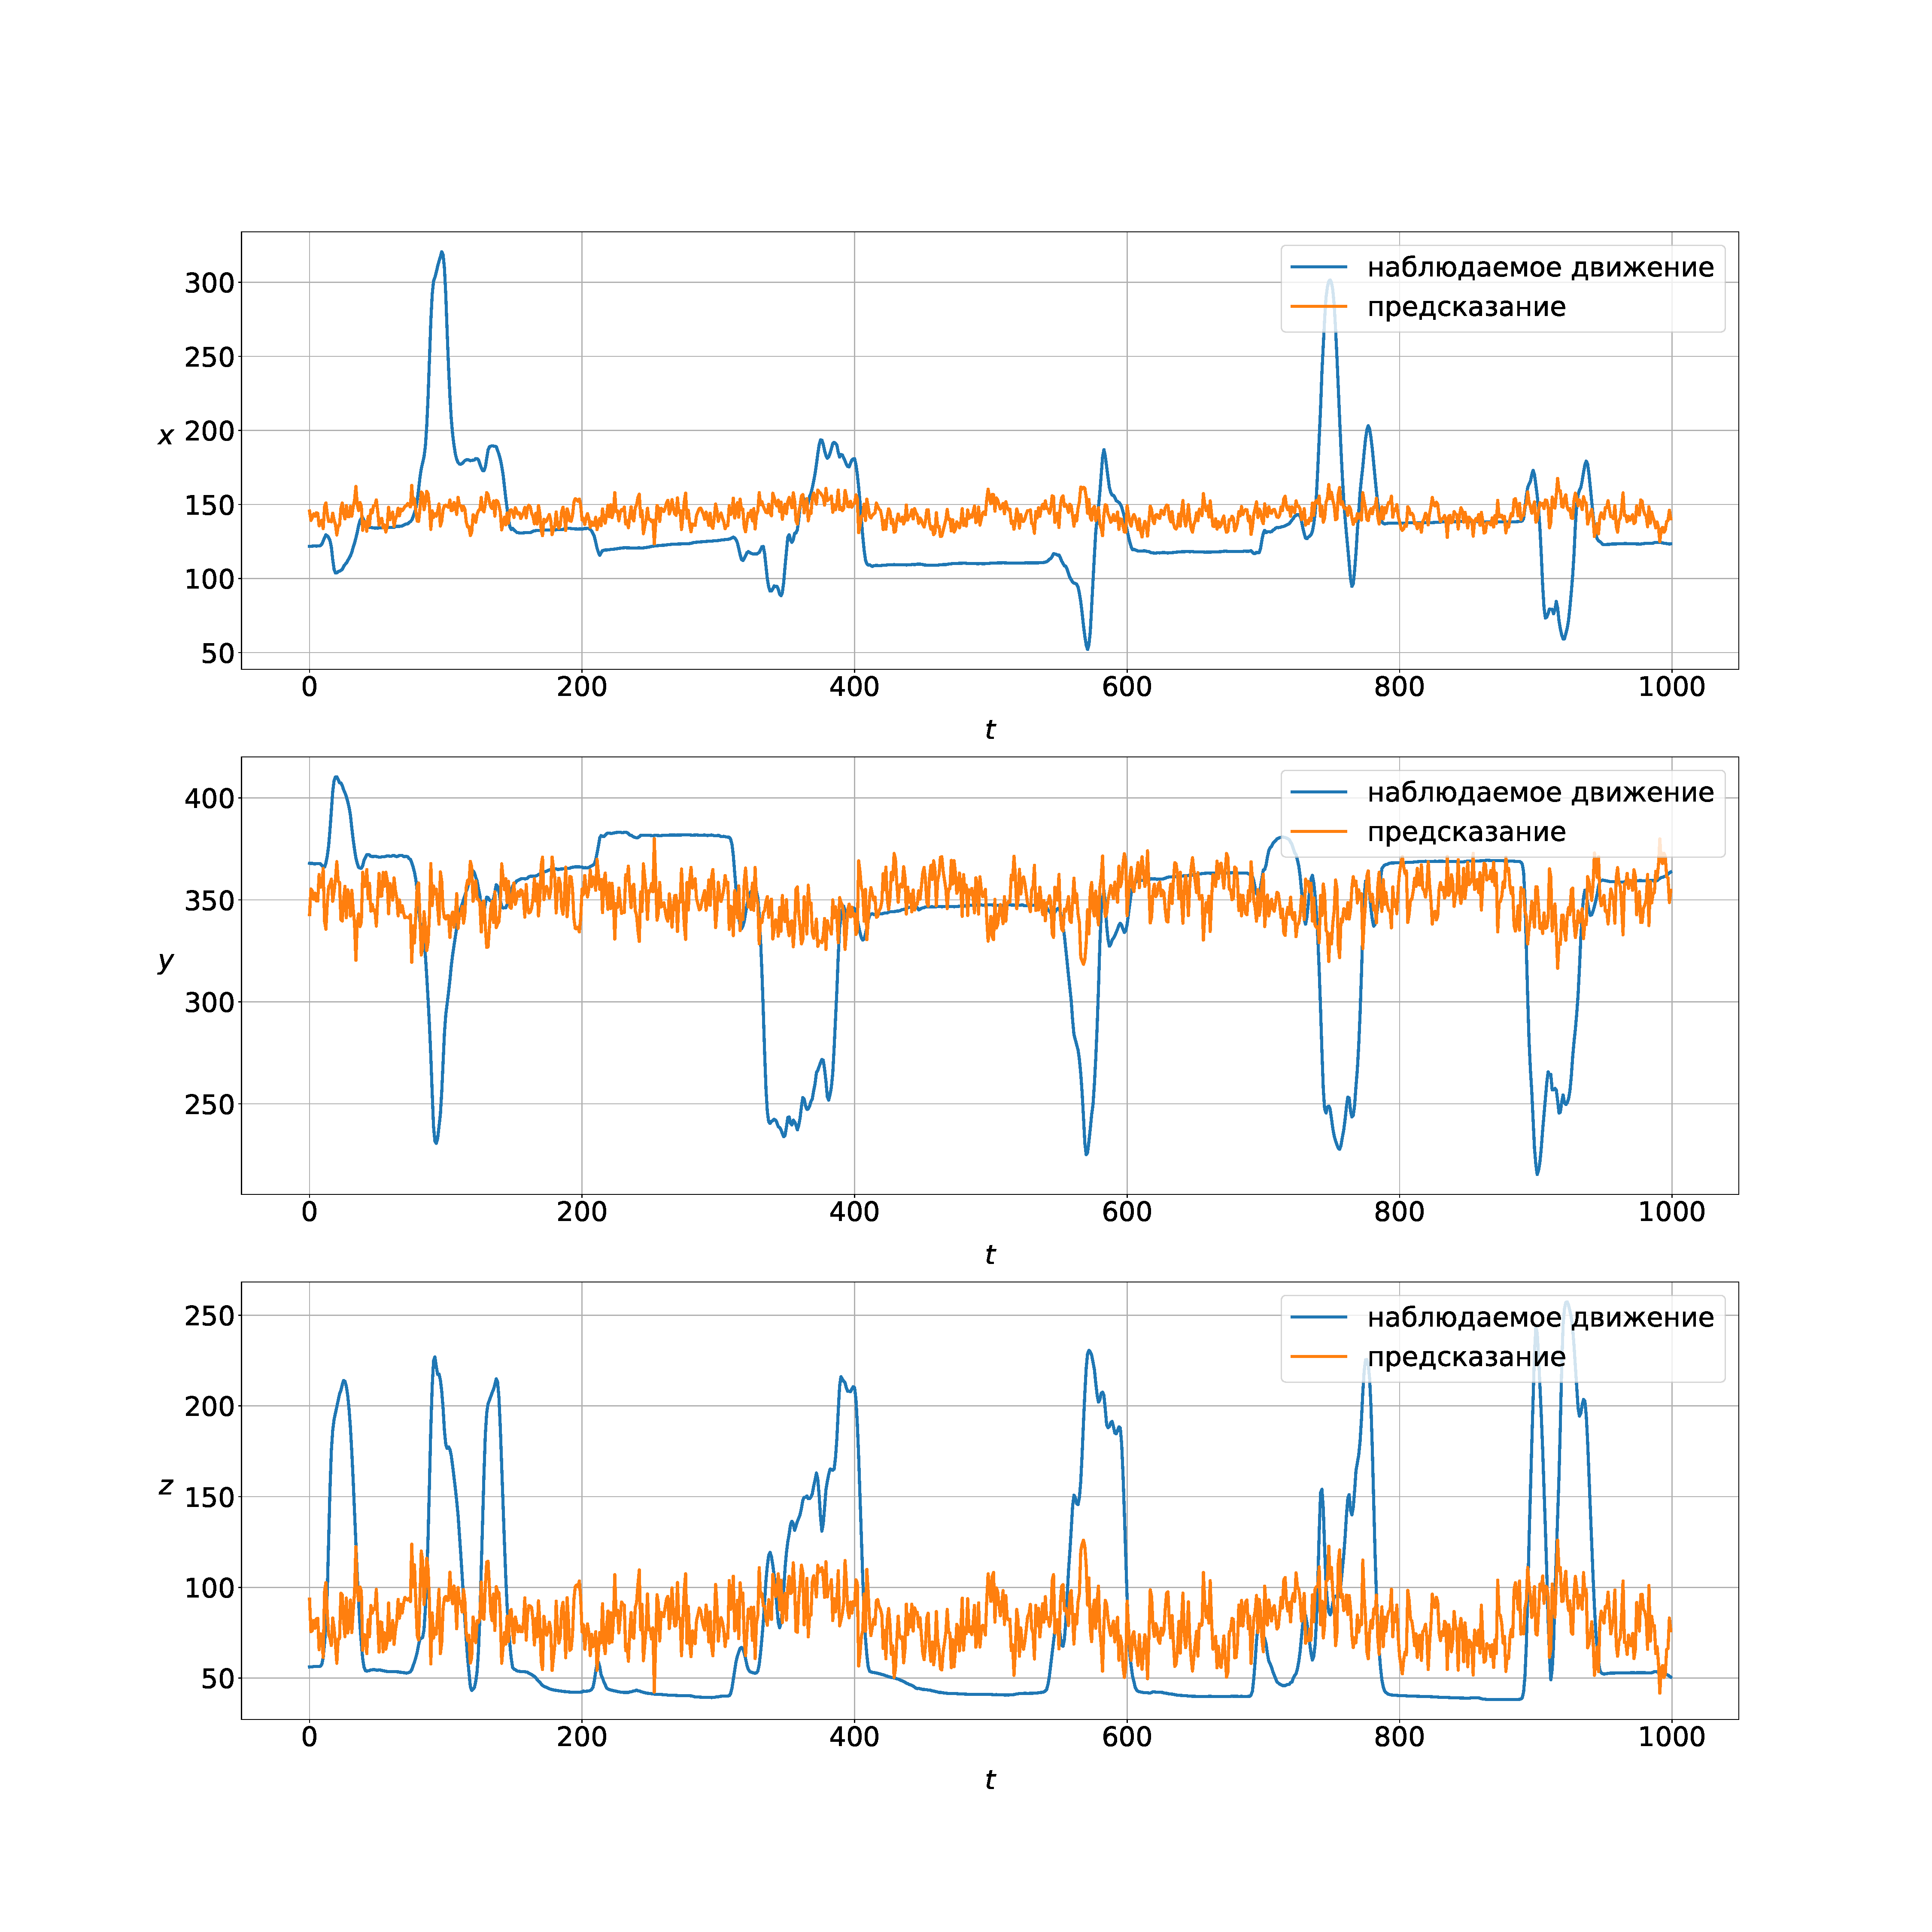
\includegraphics[width=\textwidth]{base_algo.pdf}
    \caption{Предсказания двухкомпонентного PLS, обученного на исходных данных}
    \label{fig:baseAlgo}
  \end{center}
\end{figure}
На графике представлена зависимость координаты конечности от времени. Как видно из рисунка, базовый алгоритм довольно плохо справляется с поставленной задачей. Общий профиль пиков соблюдается, однако PLS очень грубо оценивает острые пики. Также предсказание испытывает флуктуации, когда конечность почти не движется. В результате погрешность предсказания высока. Эксперимент показал значения метрик $mae = 30.17, mse = 1843.91, r2 = 0.01$. Для борьбы с погрешностями предлагается снизить размерность входного сигнала.


%\linenumbers
\bibliographystyle{unsrt}
\bibliography{../Project17}


\end{document}
